%%%%%%%%%%%%%%%%%%%%%%%%%%%%%%%%%%%%%%%%%%%%%%%%%%%%%%%%%%%%%
%
% SPAGHETTILENS -- TECH DOKU
%
% by Rafael Kueng
%
% Based on a TeXnicCenter-Template, which was
% by Christoph B�rensen, Tino Weinkauf.
%%%%%%%%%%%%%%%%%%%%%%%%%%%%%%%%%%%%%%%%%%%%%%%%%%%%%%%%%%%%%

\documentclass[a4paper,12pt]{scrartcl} %This is a special class provided by the KOMA script, which does a lot of adjustments to adapt the standard LaTeX classes to european habits, change to [a4paper,12pt,twoside] for doublesided layout


%########################### Preferences #################################


% ******** vmargin settings *********
%\usepackage{vmargin} %This give you full control over the used page arae, it maybe not the idea od Latex to do so, but I wanted to reduce to amount of white space on the page
%\setpapersize{A4}
%\setmargins{3.5cm}%			%linker Rand, left edge
					 %{1.5cm}%     %oberer Rand, top edge
           %{14.7cm}%		%Textbreite, text width
           %{23.42cm}%   %Texthoehe, text hight
           %{14pt}%			%Kopfzeilenh�he, header hight
           %{1cm}%   	  %Kopfzeilenabstand, header distance
           %{0pt}%				%Fu�zeilenhoehe footer hight
           %{2cm}%    	  %Fusszeilenabstand, footer distance         

% ********* Font definiton ************
\usepackage[T1]{fontenc}
%\usepackage[scaled=.83]{beramono}
\usepackage{lmodern}
\usepackage[utf8]{inputenc} % as usual
\usepackage[english]{babel}


% FONTS
%\usepackage{lmodern} %Type1-Schriftart f�r nicht-englische Texte
%\usepackage{mathptmx}  	%mathematical fonts for use with times, I encountered some problems using this package togather with pdftex, which I was not able to resolve

\setkomafont{disposition}{\bfseries} % chagne koma headings back


% ********* Graphics definition *******
\usepackage[pdftex]{graphicx} % required to import graphic files
\usepackage{color} %allows to mark some entries in the tables with color
%\usepackage{eso-pic} % these two are required to add the little picture on top of every page
%\usepackage{everyshi} % these two are required to add the little picture on top of every page
\renewcommand{\floatpagefraction}{0.7} %default:0.5 allows two big pictures on one page


% ********* Table layout **************
%\usepackage{booktabs}	  	%design of table, has an excellent documentation
%\usepackage{lscape}			%use this if you want to rotate the table together with the lines around the table

% ********* Caption Layout ************
%\usepackage{ccaption} % allows special formating of the captions
%\captionnamefont{\bf\footnotesize\sffamily} % defines the font of the caption name (e.g. Figure: or Table:)
%\captiontitlefont{\footnotesize\sffamily} % defines the font of the caption text (same as above, but not bold)
%\setlength{\abovecaptionskip}{0mm} %lowers the distace of captions to the figure


% ********* Header and Footer **********
% This is something to play with forever. I use here the advanced settings of the KOMA script

\usepackage{scrpage2} %header and footer using the options for the KOMA script
\renewcommand{\headfont}{\footnotesize\sffamily} % font for the header
\renewcommand{\pnumfont}{\footnotesize\sffamily} % font for the pagenumbers

%the following lines define the pagestyle for the main document
\defpagestyle{cb}{%
(\textwidth,0pt)% sets the border line above the header
{\pagemark\hfill\headmark\hfill}% doublesided, left page
{\hfill\headmark\hfill\pagemark}% doublesided, right page
{\hfill\headmark\hfill\pagemark}%  onesided
(\textwidth,1pt)}% sets the border line below the header
%
{(\textwidth,1pt)% sets the border line above the footer
{{\it University of Zurich}\hfill Rafael Kueng}% doublesided, left page
{\rmfamily Rafael Kueng\hfill{\it University of Zurich}}% doublesided, right page
{\rmfamily Rafael Kueng\hfill{\it University of Zurich}} % one sided printing
(\textwidth,0pt)% sets the border line below the footer
}

%this defines the page style for the first pages: all empty
\renewpagestyle{plain}%
	{(\textwidth,0pt)%
		{\hfill}{\hfill}{\hfill}%
	(\textwidth,0pt)}%
	{(\textwidth,0pt)%	
		{\hfill}{\hfill}{\hfill}%
	(\textwidth,0pt)}

%********** Footnotes **********
\renewcommand{\footnoterule}{\rule{5cm}{0.2mm} \vspace{0.3cm}} %increases the distance of footnotes from the text
\deffootnote[1em]{1em}{1em}{\textsuperscript{\normalfont\thefootnotemark}} %some moe formattion on footnotes


%%%%%%%%%%%%%%%%%%%%%%%%%%%%%%%%%%%%%%%%%%%%%%%%%%%%%%%%%%%%%%%%%%%%%%%%%%%%%
% my own stuff

\usepackage{amsmath}
\usepackage{xspace}   % fixes spaces after custom commands
\usepackage{float}    % exact placement of figures (using \begin{figure}[H])
\usepackage{caption}  % better captions for floats
%\usepackage{subfig}
\usepackage{subcaption} % newest package
\usepackage{fancyvrb} % for the listings


\usepackage[pdftex]{hyperref} %import last!
\usepackage{url}

\usepackage{cleveref} % used for ranges of refs

\usepackage{pgffor} % used for for loop

\usepackage{csquotes}
\usepackage[backend=biber]{biblatex}
\renewcommand{\bibliography}[1]{} % make noop. stillincl this cmd for
\bibliography{bib/bibi}           % texnicenter to display the library
\addbibresource{bib/bibi.bib}

% my macros


\newcommand{\spl}{SpaghettiLens\xspace}
\newcommand{\sw}{SpaceWarps\xspace}
\newcommand{\ml}{MasterLens\xspace}

% shortcut for einstein radius (Text Greek Full Math)
\newcommand{\ER}{Einstein radius\xspace} % text
\newcommand{\ERg}[1][]{$\Theta_\text{E#1}$\xspace} % er in textmode with greek
\newcommand{\ERf}[1][]{Einstein radius $\Theta_\text{E#1}$\xspace} % full output
\newcommand{\ERm}[1][]{\Theta_\text{E#1}} % mathmode with greek symbol

%shortcuts for kappa
\newcommand{\kenc}[1][r]{$\kappa_\text{encl}(#1)$\xspace}
\newcommand{\kap}[1][r]{$\kappa(#1)$\xspace}

% shorcuts for refs (use capital for beginning of sentence)
% first 3 are for the real layz people..
\newcommand{\fref}[1]{\ref{fig:#1}}
\newcommand{\sref}[1]{\ref{sec:#1}}
\newcommand{\tref}[1]{\ref{tab:#1}}
\newcommand{\lref}[1]{\ref{lst:#1}}
\newcommand{\uref}[1]{\ref{uml:#1}}
\newcommand{\figref}[1]{Figure~\ref{fig:#1}}
\newcommand{\secref}[1]{Section~\ref{sec:#1}}
\newcommand{\tabref}[1]{Table~\ref{tab:#1}}
\newcommand{\lstref}[1]{Listing~\ref{lst:#1}}
\newcommand{\umlref}[1]{UML~Diagram~\ref{uml:#1}}
\newcommand{\seqref}[1]{Figure~\ref{seq:#1}}
\newcommand{\Figref}[1]{Figure~\ref{fig:#1}}
\newcommand{\Secref}[1]{Section~\ref{sec:#1}}
\newcommand{\Tabref}[1]{Table~\ref{tab:#1}}
\newcommand{\Lstref}[1]{Listing~\ref{lst:#1}}
\newcommand{\Umlref}[1]{UML~Diagram~\ref{uml:#1}}
\newcommand{\Seqref}[1]{Figure~\ref{seq:#1}}

% reference to ranges of listings (for multipage..)
% \lstrefr[n_pages]{base filename}
\newcommand{\lstrefr}[2][1]{\crefrange{lst:#2_1}{lst:#2_#1}}
\newcommand{\Lstrefr}[2][1]{\Crefrange{lst:#2_1}{lst:#2_#1}}


% shortcut for ASW000xxxx
\newcommand{\asw}[1]{ASW000#1\xspace}

%shorcut for model (maybe link later to appendix)
% use \model{4356} for with text and
% \model[]{3456} for only number
\newcommand{\model}[2][Model~]{#1#2\xspace}

\newcommand{\code}[2]{%
\begin{listing}[!ht]%
  \centering%
  \input{code/#1}%
  \caption{#2}%
  \label{lst:#1}%
\end{listing}%
}



% insert multiple pages of code
% \codep[npages]{base file name}{caption}
\newcommand{\codep}[3][1]{%
  \foreach \index in {1, ..., #1} {%
    \code{#2_\index}{#3 (page \index\xspace of #1)}
  }%
}

\newcommand{\uml}[3][width=\textwidth]{%
\begin{figure}[!ht]%
  \centering%
  \includegraphics[#1]{uml/#2.pdf}%
  \caption{#3}%
  \label{uml:#2}%
\end{figure}%
}


\newcommand{\fig}[3][width=\figwidth]{%
\begin{figure}[!ht]%
  \centering%
  \includegraphics[#1]{fig/#2.pdf}%
  \caption{#3}%
  \label{fig:#2}%
\end{figure}%
}

\newcommand{\seq}[3][width=\textwidth]{%
\begin{figure}[!ht]%
  \centering%
  \includegraphics[#1]{seq/#2.pdf}%
  \caption{#3}%
  \label{seq:#2}%
\end{figure}%
}

% small code fragments

% class / object name
\newcommand{\C}[1]{%
\protect\path{#1}%
}
%method
\newcommand{\M}[1]{%
\protect\path{#1}%
}
% function
\newcommand{\F}[1]{%
\protect\path{#1}%
}
% some other code
\newcommand{\T}[1]{%
\protect\path{#1}%
}
% strings
\newcommand{\str}[1]{%
{\ttfamily "#1"}%
}
% events
\newcommand{\E}[2][]{%
\protect\path{#2[#1]}%
}

% interface
\newcommand{\I}[1]{{\ttfamily/#1/}}


% code names, LMT obejcts and classes
\newcommand{\lmt}[1]{\C{LMT.#1}\xspace}
\newcommand{\lmto}[1]{\C{LMT.objects.#1}\xspace}

% file names
\newcommand{\fjs}[1]{\textit{\protect\path{lmt.#1.js}}\xspace}

% file names
\newcommand{\file}[1]{\protect\path{#1}\xspace}

% file name bullet
\newcommand{\fbul}[2]{\item\textbf{\protect\path{#1}}\\#2}

% shell command
\newcommand{\cmd}[1]{{\\\ttfamily\$\xspace#1\xspace}}


\DeclareUrlCommand\path{\urlstyle{tt}}

% url to spaghettilens
\newcommand{\splurl}[1][]{\url{http://mite.physik.uzh.ch/#1}}


% backend stuff

%backend filename
\newcommand{\befn}[1]{\protect\path{/backend/#1}\xspace}

%database table
\newcommand{\dbtable}[1]{{\ttfamily #1}\xspace}
\newcommand{\dbfield}[1]{{\ttfamily #1}\xspace}





%%% STANDART LAENGENANGABEN %%%%%%%%%%%%%%%%%%%%%%%%%%%%%%%%%%%%%%%%%%%%%%%%%%%
\newlength{\figwidth}
\setlength{\figwidth}{0.8\textwidth}





\makeatletter
\def\PYG@reset{\let\PYG@it=\relax \let\PYG@bf=\relax%
    \let\PYG@ul=\relax \let\PYG@tc=\relax%
    \let\PYG@bc=\relax \let\PYG@ff=\relax}
\def\PYG@tok#1{\csname PYG@tok@#1\endcsname}
\def\PYG@toks#1+{\ifx\relax#1\empty\else%
    \PYG@tok{#1}\expandafter\PYG@toks\fi}
\def\PYG@do#1{\PYG@bc{\PYG@tc{\PYG@ul{%
    \PYG@it{\PYG@bf{\PYG@ff{#1}}}}}}}
\def\PYG#1#2{\PYG@reset\PYG@toks#1+\relax+\PYG@do{#2}}

\def\PYG@tok@gd{\def\PYG@tc##1{\textcolor[rgb]{0.63,0.00,0.00}{##1}}}
\def\PYG@tok@gu{\let\PYG@bf=\textbf\def\PYG@tc##1{\textcolor[rgb]{0.50,0.00,0.50}{##1}}}
\def\PYG@tok@gt{\def\PYG@tc##1{\textcolor[rgb]{0.00,0.25,0.82}{##1}}}
\def\PYG@tok@gs{\let\PYG@bf=\textbf}
\def\PYG@tok@gr{\def\PYG@tc##1{\textcolor[rgb]{1.00,0.00,0.00}{##1}}}
\def\PYG@tok@cm{\let\PYG@it=\textit\def\PYG@tc##1{\textcolor[rgb]{0.25,0.50,0.50}{##1}}}
\def\PYG@tok@vg{\def\PYG@tc##1{\textcolor[rgb]{0.10,0.09,0.49}{##1}}}
\def\PYG@tok@m{\def\PYG@tc##1{\textcolor[rgb]{0.40,0.40,0.40}{##1}}}
\def\PYG@tok@mh{\def\PYG@tc##1{\textcolor[rgb]{0.40,0.40,0.40}{##1}}}
\def\PYG@tok@go{\def\PYG@tc##1{\textcolor[rgb]{0.50,0.50,0.50}{##1}}}
\def\PYG@tok@ge{\let\PYG@it=\textit}
\def\PYG@tok@vc{\def\PYG@tc##1{\textcolor[rgb]{0.10,0.09,0.49}{##1}}}
\def\PYG@tok@il{\def\PYG@tc##1{\textcolor[rgb]{0.40,0.40,0.40}{##1}}}
\def\PYG@tok@cs{\let\PYG@it=\textit\def\PYG@tc##1{\textcolor[rgb]{0.25,0.50,0.50}{##1}}}
\def\PYG@tok@cp{\def\PYG@tc##1{\textcolor[rgb]{0.74,0.48,0.00}{##1}}}
\def\PYG@tok@gi{\def\PYG@tc##1{\textcolor[rgb]{0.00,0.63,0.00}{##1}}}
\def\PYG@tok@gh{\let\PYG@bf=\textbf\def\PYG@tc##1{\textcolor[rgb]{0.00,0.00,0.50}{##1}}}
\def\PYG@tok@ni{\let\PYG@bf=\textbf\def\PYG@tc##1{\textcolor[rgb]{0.60,0.60,0.60}{##1}}}
\def\PYG@tok@nl{\def\PYG@tc##1{\textcolor[rgb]{0.63,0.63,0.00}{##1}}}
\def\PYG@tok@nn{\let\PYG@bf=\textbf\def\PYG@tc##1{\textcolor[rgb]{0.00,0.00,1.00}{##1}}}
\def\PYG@tok@no{\def\PYG@tc##1{\textcolor[rgb]{0.53,0.00,0.00}{##1}}}
\def\PYG@tok@na{\def\PYG@tc##1{\textcolor[rgb]{0.49,0.56,0.16}{##1}}}
\def\PYG@tok@nb{\def\PYG@tc##1{\textcolor[rgb]{0.00,0.50,0.00}{##1}}}
\def\PYG@tok@nc{\let\PYG@bf=\textbf\def\PYG@tc##1{\textcolor[rgb]{0.00,0.00,1.00}{##1}}}
\def\PYG@tok@nd{\def\PYG@tc##1{\textcolor[rgb]{0.67,0.13,1.00}{##1}}}
\def\PYG@tok@ne{\let\PYG@bf=\textbf\def\PYG@tc##1{\textcolor[rgb]{0.82,0.25,0.23}{##1}}}
\def\PYG@tok@nf{\def\PYG@tc##1{\textcolor[rgb]{0.00,0.00,1.00}{##1}}}
\def\PYG@tok@si{\let\PYG@bf=\textbf\def\PYG@tc##1{\textcolor[rgb]{0.73,0.40,0.53}{##1}}}
\def\PYG@tok@s2{\def\PYG@tc##1{\textcolor[rgb]{0.73,0.13,0.13}{##1}}}
\def\PYG@tok@vi{\def\PYG@tc##1{\textcolor[rgb]{0.10,0.09,0.49}{##1}}}
\def\PYG@tok@nt{\let\PYG@bf=\textbf\def\PYG@tc##1{\textcolor[rgb]{0.00,0.50,0.00}{##1}}}
\def\PYG@tok@nv{\def\PYG@tc##1{\textcolor[rgb]{0.10,0.09,0.49}{##1}}}
\def\PYG@tok@s1{\def\PYG@tc##1{\textcolor[rgb]{0.73,0.13,0.13}{##1}}}
\def\PYG@tok@sh{\def\PYG@tc##1{\textcolor[rgb]{0.73,0.13,0.13}{##1}}}
\def\PYG@tok@sc{\def\PYG@tc##1{\textcolor[rgb]{0.73,0.13,0.13}{##1}}}
\def\PYG@tok@sx{\def\PYG@tc##1{\textcolor[rgb]{0.00,0.50,0.00}{##1}}}
\def\PYG@tok@bp{\def\PYG@tc##1{\textcolor[rgb]{0.00,0.50,0.00}{##1}}}
\def\PYG@tok@c1{\let\PYG@it=\textit\def\PYG@tc##1{\textcolor[rgb]{0.25,0.50,0.50}{##1}}}
\def\PYG@tok@kc{\let\PYG@bf=\textbf\def\PYG@tc##1{\textcolor[rgb]{0.00,0.50,0.00}{##1}}}
\def\PYG@tok@c{\let\PYG@it=\textit\def\PYG@tc##1{\textcolor[rgb]{0.25,0.50,0.50}{##1}}}
\def\PYG@tok@mf{\def\PYG@tc##1{\textcolor[rgb]{0.40,0.40,0.40}{##1}}}
\def\PYG@tok@err{\def\PYG@bc##1{\fcolorbox[rgb]{1.00,0.00,0.00}{1,1,1}{##1}}}
\def\PYG@tok@kd{\let\PYG@bf=\textbf\def\PYG@tc##1{\textcolor[rgb]{0.00,0.50,0.00}{##1}}}
\def\PYG@tok@ss{\def\PYG@tc##1{\textcolor[rgb]{0.10,0.09,0.49}{##1}}}
\def\PYG@tok@sr{\def\PYG@tc##1{\textcolor[rgb]{0.73,0.40,0.53}{##1}}}
\def\PYG@tok@mo{\def\PYG@tc##1{\textcolor[rgb]{0.40,0.40,0.40}{##1}}}
\def\PYG@tok@kn{\let\PYG@bf=\textbf\def\PYG@tc##1{\textcolor[rgb]{0.00,0.50,0.00}{##1}}}
\def\PYG@tok@mi{\def\PYG@tc##1{\textcolor[rgb]{0.40,0.40,0.40}{##1}}}
\def\PYG@tok@gp{\let\PYG@bf=\textbf\def\PYG@tc##1{\textcolor[rgb]{0.00,0.00,0.50}{##1}}}
\def\PYG@tok@o{\def\PYG@tc##1{\textcolor[rgb]{0.40,0.40,0.40}{##1}}}
\def\PYG@tok@kr{\let\PYG@bf=\textbf\def\PYG@tc##1{\textcolor[rgb]{0.00,0.50,0.00}{##1}}}
\def\PYG@tok@s{\def\PYG@tc##1{\textcolor[rgb]{0.73,0.13,0.13}{##1}}}
\def\PYG@tok@kp{\def\PYG@tc##1{\textcolor[rgb]{0.00,0.50,0.00}{##1}}}
\def\PYG@tok@w{\def\PYG@tc##1{\textcolor[rgb]{0.73,0.73,0.73}{##1}}}
\def\PYG@tok@kt{\def\PYG@tc##1{\textcolor[rgb]{0.69,0.00,0.25}{##1}}}
\def\PYG@tok@ow{\let\PYG@bf=\textbf\def\PYG@tc##1{\textcolor[rgb]{0.67,0.13,1.00}{##1}}}
\def\PYG@tok@sb{\def\PYG@tc##1{\textcolor[rgb]{0.73,0.13,0.13}{##1}}}
\def\PYG@tok@k{\let\PYG@bf=\textbf\def\PYG@tc##1{\textcolor[rgb]{0.00,0.50,0.00}{##1}}}
\def\PYG@tok@se{\let\PYG@bf=\textbf\def\PYG@tc##1{\textcolor[rgb]{0.73,0.40,0.13}{##1}}}
\def\PYG@tok@sd{\let\PYG@it=\textit\def\PYG@tc##1{\textcolor[rgb]{0.73,0.13,0.13}{##1}}}

\def\PYGZbs{\char`\\}
\def\PYGZus{\char`\_}
\def\PYGZob{\char`\{}
\def\PYGZcb{\char`\}}
\def\PYGZca{\char`\^}
\def\PYGZsh{\char`\#}
\def\PYGZpc{\char`\%}
\def\PYGZdl{\char`\$}
\def\PYGZti{\char`\~}
% for compatibility with earlier versions
\def\PYGZat{@}
\def\PYGZlb{[}
\def\PYGZrb{]}
\makeatother



\newfloat{listing}{tbhp}{lst}[section]
\floatname{listing}{Listing}
\newcommand{\listoflistings}{\listof{listing}{List of Listings}}

%\newsubfloat{listing}



%\makeatletter
%\newbox\sf@box
%\newenvironment{SubFloat}[2][]%
%{\def\sf@one{#1}%
%\def\sf@two{#2}%
%\setbox\sf@box\hbox
%\bgroup}%
%{ \egroup
%\ifx\@empty\sf@two\@empty\relax
%\def\sf@two{\@empty}
%\fi
%\ifx\@empty\sf@one\@empty\relax
%\subfloat[\sf@two]{\box\sf@box}%
%\else
%\subfloat[\sf@one][\sf@two]{\box\sf@box}%
%\fi}
%\makeatother



%\newfloat{sublisting}{tbhp}{lst}[listing]
%\floatname{sublisting}{MultiPageListing}
%\newcommand{\listofmplistings}{\listof{sublisting}{List of MPListings}}
%\newsubfloat{sublisting}

%################ End Preferences, Begin Document #####################

\pagestyle{plain} % on headers or footers on the first page

\begin{document}

\begin{figure}[th]
    %\centering
		
\includegraphics[width=5cm]{pic/uzh}
	\label{fig:logo}
\end{figure}

\begin{center}

\vspace{0.5cm}


{\Huge\bf SpaghettiLens\\}
\vspace{0.5cm}
{\Huge\bf ---\\}
\vspace{0.5cm}
{\Huge\bf Lens modeling made easy}

\vspace{2cm}

{\Large\bf Master's Thesis}

\vspace{1cm}

{\Large\bf Presented for:\\}
{\Large Master's Degree in\\}
{\Large Computational Science\\}
{\Large from the\\}
{\Large University of Zurich\\}

\vspace{1cm}

{\Large\bf Presented by:\\}
{\Large Rafael Küng\\}

\vspace{1cm}

{\Large\bf Supervised by:\\}
{\Large Dr. Prasenjit Saha\\}
{\Large Prof. Dr. George Lake\\}


\vspace{1cm}

{\Large Zurich, September 2013} 

\end{center}
\newpage

\pagestyle{cb} % now we want to have headers and footers

\tableofcontents
\newpage

\section{Introduction}

Gravitational lenses (GLs) are a great tool for astronomers to study properties of the cosmos.
But before they can be used for further studies, they have to be spotted.

This is a hard task, given the huge amount of data which observatories produce and the average performance of existing robotic lens detection tools.
\sw\footnote{\protect\url{http://www.spacewarps.org}} addresses this problem by inviting volunteers to help spot GLs, with a great success.
Over 1.7 million images have been classified in the first two weeks after the start of the citizen science project.

The next step is to analyze and model the lens candidates found.
A convincing model for a lens candidate supports the hypothesis that it is really a lens. Further, it is the first step in a more detailed analysis of the lens.
It allows for example the analysis of the matter distribution including dark matter.

Creating a model is a rather sophisticated, time intensive task usually done by scientists.
We proposed that it is possible for non scientists (volunteers\footnote{also known as citizen scientists}) to create models that are comparable to those of scientist. This requires in a first step to present the underlying theory in a compact and simple way.
Second, a modeling tool has to be developed that simplifies the process of creating a model.
It would be preferable, if this tool provides an instant, meaningful visual output.
That would allow the volunteers to improve their models iteratively, by try and error.
In a third step, the building of a community of users should be encouraged.
On one side by closely working together to further adjust the tool to the users needs, on the other side to assist if any questions come up.


This report introduces the tool written for this task: \spl.
It was part of the authors Master Thesis and details the design and set up of the tool.
This is intended to be a technical documentation for anybody who wants to understand and contribute to the application.

The scientific part of my Master Thesis is to test our proposal by letting volunteers model simulated lenses.
The known parameters of the simulations were compared to the parameters of the models generated by the volunteers.
The results of this part can be found in the scientific paper (to be published, you can have a look at the draft at \url{http://www.physik.uzh.ch/~rafik/?f=slp.pdf})

Additionally, a tutorial video was recorded, which explains the theory and use of \spl\footnote{\protect\url{http://mite.physik.uzh.ch/tutorial/}}.


%, a tutorial homepage giving written explanation of whats shown in the video and a sub page for \sw called labs, where different modelng tools will be collected and presented. The last two are not yet online.

\subsection{\spl}

\spl is build around GLASS\cite{glass-jc}, a non parametric, pixel based lens modeling tool set.
GLASS is a reimplemented version of PixeLens\cite{pixelens}
%
\spl is build as a client-server web application, that runs on any computer in the browser without any installation\footnote{Besides an up to date browser}.
If offers the following features:
\begin{itemize}
  \item Quickly create models of lenses, originating from different data sources (\sw, \ml \footnote{\protect\url{http://www.masterlens.org}})
  \item Users can easily present their results, discuss and improve them
  \item Allows scientists to store, manage and evaluate models and data for lenses
\end{itemize}

It was designed using modern web technologies to implement a powerful, modular web application.
Chapter \ref{sec:primer} gives an introduction to current web technologies applied in this project.
The main part of this report is Chapter~\ref{sec:setup}, explaining all the parts \spl is made of in detail, whereas Chapter~\ref{sec:pd_flow} details the interplay between the modules.
Chapter~\ref{sec:deployment} gives a short overview over the installation and maintenance and finally some review and outlook in Chapter~\ref{sec:outlook}.



\clearpage
\section{Primer in Web Technologies}

This section gives a short overview over the techniques and standards used in web development.
It introduces the concept of 


\subsection{HyperText Markup Language (HTML)}
The HyperText Markup Language (HTML) is the markup language used as a format to exchange semantically structured information on the internet.
It is a textual language describing the building blocks of a web site.
Those building blocks are called tags.
They are enclosed in angle brackets and consist of opening tag, a set of attributes like id, class and additional depending on the tag type, and an closing tag, see \lstref{atag.html}

\code{atag.html}{Example HTML tag.}

This tags can enclose any content, data to be displayed or other tags. This results in an document tree, that can be accessed using the interface ``Document Object Model'' (DOM). Often, the document tree itself is called DOM\footnote{DOM describes actually an interface, not a model.}.



\subsection{Cascading Style Sheets (CSS)}

\subsection{ECMAScript (aka JavaScript JS)}

\subsection{Dynamic HTML (DHTML)}

\subsection{Server side scripts}

\subsection{Asynchronous JavaScript and XML (AJAX)}

\subsection{Server communication}

\subsection{Graphics -- HTML images vs HTML5 canvas vs Scalable Vector Graphics (SVG)}
To produce a webapp, often a custom user interface and output display is needed.
HTML in combination with CSS and static images offer only very limited abilities, to design a custom dynamic screen elements.
Scalable Vector graphics (SVG) and HTML5 canvas offer more powerful techniques to create dynamic screen content.

\subsubsection{HTML images}
All HTML DOM elements are rectangles and can be placed anywhere on the screen using CSS.
This includes the image tag \T{<img>}, that allows a set of images to be composed to an interface.
JS can be used to change the position of DOM elements, or change the image file they display.
But HTML4 offers no abilities to change the contents of a particualr image, meaning you have to create all the images that possibly could be displayed.
This is fine for simple setup like a menu, but for an advanced user interface, this is not practical.

\subsubsection{HTML5 canvas}
The HTML5 specification defines a new tag, called Canvas \T{<canvas>}.
It allows pixel based image manipulation, by offering a canvas that consists of a discrete, rasterized 2D array of pixels.
By using JS, each pixel of this image grid can be accessed and it's color can be changed dynamically.
There are helper functions that allow the drawing of lines, shapes, paths and images.

Canvas offers fast, low level pixel wise image manipulation.
It is ideal for image manipulation on a per pixel basis like blending.

It offers no scene graph, that keeps track of which structures and shapes were used to draw on the canvas.
If one element changes its position, the canvas needs to be deleted and all objects need to be painted again.
The canvas offers JS callbacks for user actions like click, returning the coordinates of the pixel that was clicked on.
The programmer has to implement a scene graph himself if he wants to know what object / element was clicked on.

\subsubsection{Scalable Vector Graphics (SVG)}
Scalable Vector Graphics (SVG) is a vector image format standard, using a markup language (similar to HTML, based on XML).
SVG defines a continuous coordinate system, on which mathematical constructs are defined on.
This mathematical constructs are objects like paths, basic shapes, test, raster graphics, that are directly stored as a SVG tag in the SVG file.
Since SVG is an XML language, it is comparable with HTML.
CSS can be used to define styles for the SVG objects and JS can be used to manipulate properties.

SVG files offer high level access to graphics, based on shapes.
The direct access to shapes with JS makes it easy to dynamically modify elements or add new shapes.
The SVG DOM can be directly included in the HTML DOM, offering unified access from JS to all HTML and SVG objects.
JS events get fired like in regular HTML.
For example each shape fires an \T{onClick} event if clicked on.


By design, SVG is slower as canvas, because it first needs to rasterized by the browser in order to be drawn on the screen.
Additionally, there was put a lot of effort in Canvas optimization and hardware acceleration lately, whereas SVG hardware support is only minimal.
Due to the lack of hardware optimization, pixel based operations like filters operate slowly.







\clearpage
\section{Implementation of \spl}
\label{sec:setup}



\spl applies the concept of an AJAX web application, as described in \secref{ajax}.
It consists of several modules communication through defined APIs.
\figref{whole_setup} shows an overview of the implemented modules and their communication channel.

\begin{figure}[htbp]
  \centering
    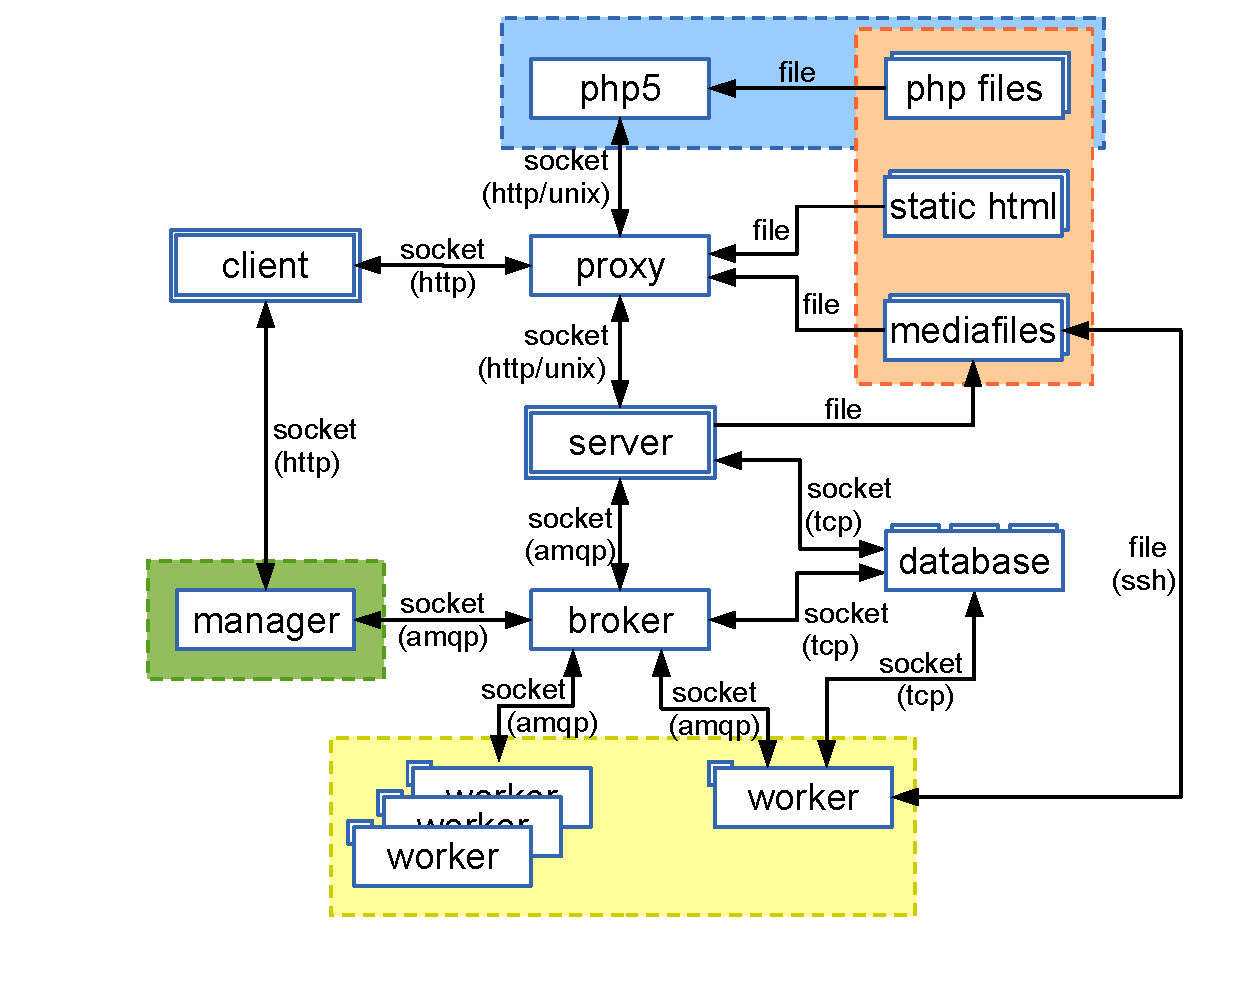
\includegraphics[width=\textwidth]{fig/whole_setup.pdf}
  \caption{\spl setup. The modules and their communication.}
  \label{fig:whole_setup}
\end{figure}


%This section elaborates the implementation of \spl by explaining design consideration and implementation details for all the modules.
\Figref{whole_setup} shows all modules used in the current setup as an web application at \splurl.
The client, server and worker modules are the core components, needed to run \spl.
Other setups are possible, \spl could also run as a native desktop application using only the core modules set up differently.

One advantage of this modularized approach is the scalability of the application.
Each module can possibly run on it's own hardware, in case the use of the application increases.

The application features a simple flow of data.
After the loading of a Lens into the client application on the browser (client), the user creates a model, represented as a JSON string.
This model is sent to the server side application, there the model and all according parameters are saved in a data base.
Additionally, the server creates a configuration file (\T{.cfg} file) stored in the file system for the simulation application (worker) to run on.
The worker runs the simulation and the resulting set of models is saved to the file system as a State file (\T{.state}).
A second worker type (renderer) then loads this state file and creates the resulting images (mediafiles) and saves them to the file system.
In the current implementation, the simulation and the rendering are done by the same worker.
Future development will feature a separate renderer, to allow the creation of arbitrary plots from already simulated data.
In a last step, the client loads the rendered images to give the user a visual feedback of the model created.
\Figref{dataflow} shows this high level view of data flow.
The sections in this chapter elaborate the interfaces for this data flow, the design of according data structures, as well as the mechanics and implementation of the modules.
\Secref{pd_flow} shows the program and data flows more detailed.

\begin{figure}[htbp]
  \centering
    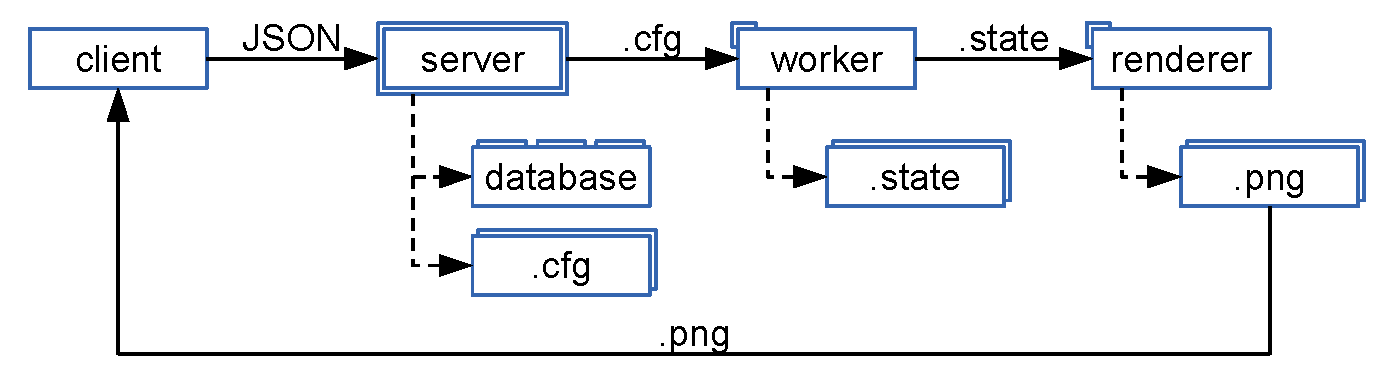
\includegraphics[width=\figwidth]{fig/dataflow.pdf}
  \caption{High level view of flow of data involved in creating a model and data objects saved.}
  \label{fig:dataflow}
\end{figure}




\clearpage
\subsection{Client}
\label{sec:client}

\subsubsection{Overview}
\label{sec:client_overview}


\subsubsection{Techniques}
\label{sec:client_techniques}



In webapp programming, is basically an interactive webpage, that communicates with other components.

To accive that, you need 3 technologies: html, css and javascript. This is a unique standart.

HTML describes the logical structre and layout of your webpage, the userinterface. That elements are on the page.

CSS defines the visuals, optics. how those elements defined by HTML are displayed. How those elements on the page look like

Javascript (js) is the programming language, that runs on the client computer and thus defines the behaviour. It describes, how the elemnts interact with each other.


\spl was designed to do as much computation as possible on the client side.
This removes the load on the application server, network traffic and leads to a more natural feeling.
The app responds instantaniouly to user inputs (instead of having to wait for a server response).
Drawback: you have less control over data (saving snapshots) since browser are usually encapsulated from the rest of the computer, difficult to save status / data client side.


An interactive webpage / user interface needs javascript for document object model (DOM, the tree of html attributes describing the structre of the webpage) manupulation.
\spl consists of a single website.
In opposite to most classical websites, where you click a link and load another page to react to user input, \spl is only one single page, that updates it's strucrte live as the user interacts with the page (called DHTML, dynamic HTML).
Thus a dhtml webpage resembles more a classical desktop application than a classical website.

If your DHTML site needs to exchange information with a server (e.g. to do some heavy calculations, store and retrieve data from a central database) you get Ajax (Asynchronous JavaScript and XML).




ECMAScript (aka JavaScript)


The modern webapp has thus 4 components: user input, output, intelligence, communications.
All of which is programmed in javascript.
Since this is a very common task, there are several libraries implemented in javascript, that facilitate the DOM manipulation (and thus creating a user interface).

For \spl the the most common one was chosen, jQuery.
It is used by two thirds of the top 10'000 webpages.
It is open source and due to it's widespread use, it guarantees to be kept up to date and get often bugfixes.

jQuery offers several addons, one of them jQuery UI, that facilitates the einheitliches design of user interfaces

basically, jquery makes it easy to find, access and modify elements in the DOM, as shows \lstref{jquery_vs_js.js}.

\code{jquery_vs_js.js}{Comparing the modification of some objects, done in jQuery and pure js.}




HTML

There are two versions of html: the actual version 4.01, which almost anything that is connected to the internet is compatible to, probably even you toaster. Version 4 is around since Dec. 1998.

And the next generation HTML5, that is currently in developpent (First working draft from Jan 2008).
It offers many new features, for audio, video and graphics (canvas), communications (websockets), local storage.
But is only supported by newer Web Browser and thus a smaller user base.

Never the less we decided to go for html5. Because if offers the canvas and svg, two essential techniques explaned later for a web app.
Since our expected user base will origin from galaxzoo and \sw, and those sites are also programmed in HTML5, we could expect our users to have up to date browsers.



\subsubsection{Visual Layout}
\label{sec:client_vis_layout}

The User Interface was designed to be as simple as possible.
It should hide away all settings that are not needed by default.
To be self explanatory is almost impossible given the problem.
Users will need to see a tutorial anyways.

The basic degin idea was to provide a visual feedback and easy comparison between the input modelling parameter and the resulting output model.
This is accived by putting the input area and output area side by side.
All the functions that the user needs to manupulate the input are arranged on top of it, everything manipulating the output above the output window.
A few general commands are arranged in a top bar.

To assist the user, two systems are present: A exhaustive mouse over hoover tooltip help that pops up any relevant information for an tool / button under the cursor.
This provides a short description of the action, and possibly a link to athe tutorial page.

Additionally, there is a help bar at the bottom. This can be hidden from the toolbar.
It also provides information about objects in the input area.
mouse over tooltips would not function in the input area well, obstructing the users view over the model, hence this two folded helping system.

For clients with a small screen, like mobile devices and possibly tables, the layout changes to only display the input or the output. The user can slide between those to sides using a slider.\footnote{Note that mobiles weren't tested and are not officially supported yet.}


\subsubsection{Programm Layout}
\label{sec:client_prog_layout}

The client side application was programmed with a strict object oriented and event driven perspective.
Instead of a regular program that has a main loop, that runs infinitly and where subfunctions are called, a event driven program is at halt when idle, and reacts to event that can be fired by any source (example: a key press triggers a function, instead of looping infintely and checking if any key was pressed.)
This is a very simplified abstractaion\footnote{and technically not entirely true, there is an main loop that checks if events happend and then a dispacher calls the registered function.} but describes the situation of running JavaScript in a browser quite well.

Everything is a object. The toolbar, the model, a dialogue screen.
All objects can fire events and react to events and thus change their internal state, and/or fire a subsequent event.
There are unique objects (like toolbar, input area) and instances of prototype objects\footnote{in other programming languages prototype objects are called classes}. There can be more than one instance of a prototype object (for example Extremal Points, Point masses...)

The program is always in a certain state, defined throu the attributes of all the objects. In \spl, the state consists of the state of the model, and the state of the ui.

The main part of \spl is the object lmt.events, \lstref{js__lmt.events_part.js} shows an excerpt. This object registers at startup, which objects react with witch object function on what events and thus, this object defines all events possible (except a few standard events).

\code{js__lmt.events_part.js}{An exerpt from lmt.events.js}

There are basically three groups of objects that interact with each other: The user interface objects (LMT.ui, split in LMT.ui.svg, LMT.ui.out, LMT.ui.html), the comunications object (LMT.com) and the current model (LMT.model, instance of LMT.objects.model)

A model consists of an array of sources, an array of external masses (instances of LMT.objects.ExternalMass) and an parameter object. Each source is represented by an tree structure of instances of extremalpoints (LMT.objects.ExtremalPoint)

Additionally, there is an action stack (LMT.actionstack), LMT.datasource, LMT.datasources

and some objects that only store common data / functions that needs to be accessed by multiple objects (LMT.modelData, LMT.settings, LMT.simulationResult, LMT.utils)


\uml[width=0.4\textwidth]{model}{a model}

\clearpage
\subsection{Interface Client Server}
\label{sec:iface_c_s}

interface client server

%\codep[0]{json_repr_parts.js}{The building blocks of a model in JSON notation} 
%\codep[1]{json_repr_parts.js}{The building blocks of a model in JSON notation} 
%\codep[2]{json_repr_parts.js}{The building blocks of a model in JSON notation} 

%\codep{2}{json_repr_parts.js}{The building blocks of a model in JSON notation} 

%\begin{listing}%
  %\centering%
  %\begin{SubFloat}[bla]{\label{tmp1}Capt label1}
    %\input{code/tmp1}
  %\end{SubFloat}
  %
  %
  %
%%  \subfloat[\label{tmp1}]{\input{code/json_repr_parts.js_p0}}%
%%  \caption[\label{tmp1}]{}
  %%
    %%\label{lst:tmp1}%
%\end{listing}%
%
%
%\begin{listing}%
  %\ContinuedFloat
%
  %\begin{SubFloat}[bla2]{\label{tmp2}Capt label1}
    %\input{code/tmp2}
  %\end{SubFloat}
%
%
  %%\centering%
  %%\subfloat[\label{tmp2}]{\input{code/tmp1}}%
  %%\input{code/tmp2}%
  %%\caption[\label{tmp1}]{}
  %}%
  %%\label{lst:tmp2}%
%\end{listing}%



%\codep[0]{json_repr_parts.js}{The building blocks of a model in JSON notation} 
%\codep[1]{json_repr_parts.js}{The building blocks of a model in JSON notation} 



%\cref{lst:json_repr_parts.js_1,lst:json_repr_parts.js_2,lst:json_repr_parts.js_3}

The server offers three points to exchange data: \I{api}, \I{tools} and \I{data}.

Since there is some legacy code still in the code base, there are additional, depreciated url access points to exchange data. (\I{get\_initdata}, \I{get\_modeldata}, \I{save\_model}, \I{save\_model\_final}, \I{load\_model}, \I{result})

\I{api} is supposed to handle all communication with the client application.
The client can do a HTTP POST request to \splurl[api].
The requests body should contain at least the key \str{action} set to the value of the desired action.
The basic transmission format is JSON based.
Depending on the action chosen, additional key/value pairs need to be transmitted.
Have a look at the source code files \befn{ModellerApp/views.py} and/or \fjs{com} for details.



\codep[3]{json_repr_parts.js}{The building blocks of a model in JSON notation} 


\Lstrefr[3]{json_repr_parts.js} shows the JSON communication format for sending models between client and server in a structured notation. This has the same tree like structure as is shown in \umlref{model}.


\I{data} offers an access point, to present simulated models in an easy way.
It answers to a basic HTTP GET request by parsing the rest of the url to a integer result id and returning a simple web page showing this result number.
\splurl[<result-id>]\footnote{example: \splurl[1337]}


\I{tools} offers access for advanced users and admins to tools for administering collaborative modeling, getting more detailed data ect.
At the moment, only one tool is implemented: \I{tools/ResultDataTable}.
This tool creates an overview table over all parameters for a set of result ids.
The resulting table can be downloaded as a Excel file (\T{csv}) or directly shown in a browser (\T{HTML-table}).
The query to the data base is directly composed of the HTTP GET parameters:
\splurl[tools/ResultDataTable?6696,6904-7000\&type=html].
For a full documentation visit the tool without any argument\footnote{\splurl[tools/ResultDataTable]}.







\clearpage
\subsection{Proxy}
\label{sec:proxy}

In the current setup, there is a proxy server between the application server and the internet.
It's purpose is to reduce the load of the application server and prevent the firing up of a resource intensive\footnote{CPU time and memory size} python thread in the app server on every request.

It is supposed to directly serve the client application. Further, this particular server is set up to serve \url{labs.spacewarps.com} and the \spl documentation and tutorial page in combination with a php process.\footnote{this part is still work in progress}

It is setup to further intercept requests to \I{data} and return the data directly, if available.
Only if the result first needs to be rendered, it is passed on to the application server.

It is also set up to cache any requests made to \I{api} that can be regarded as static, like getting the information about a lens.

At the moment, the proxy uses the web server software nginX (``Engine X'') that is preferred over Apache because of the small memory finger print.
This is due to the fact that nginX is event based, in opposite to Apache, which is process based.
nginX is often used as proxy server and load balancer to serve static content infront of other server like apache that handle the dynamic content.




\clearpage
\subsection{Server-side Scripts (Server)}
\label{sec:server}

As explained in \secref{serverside}, the server application is basically an interface to the database.
\spl splits the server-side scripts further up and distinguishes between the module that manages data (server) and the part that generates data (worker) that is introduced in \secref{worker}.

The server manages all the data needed and generated by the client app.
It keeps track of lenses that can be modeled (\T{LensData} objects identified by \T{model_id}\footnote{Will be renamed to \T{lens_id}.}), create new ones from the data sources available, created models (\T{ModellingResult} objects, identified by \T{result_id}) and keeps track of simulation results and files.

The server provides the client unified access to survey images hosted on several possible external data sources (at the moment, \sw is fully and \ml partially implemented).
It keeps track which models (results) belong to which lens, which user created a model and which models are descendants from each other.

Additionally, it is the interface between the client app and the workers that do the actual modeling.
It has to convert the data generated by the client (JSON) to a format that the modeling application requires (GLASS config files).


\subsubsection{Techniques used}

The server is implemented in Python language, using the Django framework.
The framework is served using gunicorn, a WSGI HTTP server implemented in Python.

The Django framework follows a ``model-view-controller'' architecture.
It defines a data model which is represented in a backend database.
A ``view'' is a representation of a subset of this data presented to a user (the client app in this case).
The ``controller'' allows to modify the data.

The data model is created by defining Python classes in \befn{ModellerApp/models.py}.
Django uses a relational database in the backend, to keep track of all the created instances of those models.
For the actual storage of the data, Django relies on a external relational database.
For \spl, MySQL, the most popular\cite{dbranking} open source database, was chosen.

Views and controllers are defined by Python functions (\befn{ModellerApp/views.py}).
Those functions get mapped to HTTP requests by \befn{lmt/urls.py}.
They process a request and either query the model / database in order to return a representation of the data or update the data.



Django offers a powerful template system that allows to render the data in any possible form.
Usually it's used to render HTML pages, but this setup uses it to return JSON data objects to the client app.
The template system is used to render the result views\footnote{\splurl[data/<result_id>]}, which can be accessed directly by a browser to display generated models.

In order to simulate the models, the server needs to connect to GLASS, the simulation software, tell it what to do and fire it up.
The server creates a config file for GLASS for each request, and then starts an instance of GLASS running this file.
Since the simulation takes in the order of minutes, the server worker process should not be blocked during simulation.
Additionally, this part should be easily scalable, since it creates the biggest server load and needs to be scaled up linearly with the amount of users that use \spl concurrently.
This is done using a task distribution system (Celery) that will be introduced in \secref{worker}.







\subsubsection{The Design of the API}


\uml[width=1\textwidth]{serverapi_full}{An overview over the server API and the internal functions.\\Green background: origin of requests. Blue background: caching proxy. Yellow background: API (controller definitions). White background: internal functions. Grey background: functions to be removed in future versions.\\Lines show flow of data (function calls, HTML requests).}



\Umlref{serverapi_full} shows a complete overview of the server API.
Note that the API is currently under redesign.
The old design paradigm stated that each possible action of the server was exposed directly to an URL, where a client could make a HTTP request to. This assignment is configured in \befn{lmt/urls.py}.
It has the draw back that those access points need to be configured on the server side in two places, in the server application, and additionally in the proxy.

In the new design paradigm, there are only three access points offered. This simplifies the administration of the proxy server and increases the flexibility of the application.




\subsubsection{The Design of the Database}


\uml{db}{UML database schema. Using Django notation for field types.}

The database schema is shown in \umlref{db}.
There are two important tables in the database.
The first is the table of all lenses that have been modeled: \dbtable{LensData}.
It stores all the objects from all different data sources, as soon as they have been requested once.
It keeps track of the origin of the image in the field \dbfield{datasource}.
The location of the image files is stored in \dbfield{img\_data}, as a JSON string.
This JSON object needs at least a key \T{url}, pointing to a publically available image.
If a lens consists of multiple images (multiple filters / bands...), those can be stored in this JSON object too.\footnote{to be implemented in the client side.}
Arbitrary additional data (to be used in the corresponding datasource modules client and server side) can be stored as JSON strings in \dbfield{add\_data}.

The second table, \dbtable{ModellingResult}, keeps track of all the models that were generated.
It keeps track of the \dbtable{LensData}, of which it is a result and stores the JSON string generated by the client that represents this model in \dbfield{json\_str}.
If this result is a refined version of a previous one, the key of the previous one is saved in \dbfield{parent\_result}, which creates a tree-like structure.
Additional administration information is kept in \dbfield{created\_by}, \dbfield{rendered\_last}, \dbfield{last\_accessed}.
This information can be used for later clean up purposes`, like the deletion of the modeling state files and rendered images for models that are not visited anymore.
GLASS parameters used to generate the model are stored in the according fields.


\subsubsection{The parsing of a model JSON string}

In order to save a received model from the client app, the server parses the JSON string received and converts it to a temporarily Python data structure.
This is done in \befn{ModellerApp/utils.py}, using the class \C{EvalAndSaveJSON}.

\F{EvalAndSaveJSON.__init__()} first sets all the default values for glass and then calls \F{EvalAndSaveJSON.evalModelString()}.
This function parses the JSON model string to a Python dict containing Python objects.
The parameters of the uploaded model are then, after a sanity check, written over the default values.

In a second step, \F{EvalAndSaveJSON.orderPoints2()} reorders the tree-like structure of extremal points provided by the client to a list of images ordered by their expected arrival time. It determines the center of the lensing galaxy (assumed to be the maximum). This also converts all the measurements from \spl pixels to actual arcsec and makes them relative to the center of the lens.

The third step \F{EvalAndSaveJSON.createModellingResult()} creates the database entry in \dbtable{ModellingResult}.
The last step \F{EvalAndSaveJSON.createConfigFile()} creates the GLASS config file to be supplied to the modeling software.


\codep[2]{glass_cfg.py}{GLASS config file}









\clearpage
%\section{Interface Server Worker}
\label{sec:iface_s_w}

interface2
%\clearpage
\subsection{Worker}
\label{sec:worker}

The actual simulation of the models is done by GLASS.
Since the modeling takes in the order of minutes, a modeling task can not simply be done by the server.
Depending on the server architecture, this would block at least a web server worker thread, making it unable to respond to other requests.
Since the simulation of models is the most CPU intensive task, this needs to be easy scalable, in case more users start to use \spl. 
Preferably, the simulation jobs could be distributed to several machines.

GLASS is a command line application that expects a config file to run on.

For the management of the worker thread Celery was chosen.


\subsubsection{Celery overview}
Celery is distributed task queue implemented in Python.
It offers integration packages for many web frameworks, including Django.
This makes the setup of a distributed task system with Django and Celery easy.

\code{start_task.py}{Example of how to call a task from Django. Simplified version of \F{getSimulationJSON()} from \befn{ModellerApp/views.py}}

Possible units of work, called tasks, can be defined as python function on the server side in Django using the file \befn{/lmt/tasks.py}.
This tasks can be started by Django asynchronously by a call to the task as shown in \lstref{start_task.py} and return a \C{AsyncResult} instance that allows to check the state of the task or it's return value in a next step.

Once a task is started by Django, Celery takes over.
The task is sent to a message broker that implements the task queue.
The celery worker threads then consume the tasks from this queue, process it and save the result back in a result back end. The result backend keeps also track of the tasks states.

All these processes communicate over TCP sockets and thus can run on different machines.

\subsubsection{The tasks}

\code{tasks.py}{Server side definition of worker task. Simplified version of \befn{lmt/tasks.py}}
\code{run_worker.sh}{Shell script representing a task.}

The tasks are defined in \befn{lmt/tasks.py} on the server side.
It's a simple call for a shell script that gets the needed files, calls GLASS, and upload the results back to the servers file system.
See \lstref{tasks.py} for the definition of tasks and \lstref{run_worker.sh} for the called shell file.



\subsubsection{The message broker}

The message brokering is done with RabbitMQ, the recommended task queue backend.
It is open source software written in Erlang, implementing Advanced Message Queueing Protocoll (AMPQ).

\subsubsection{The worker threads}

Worker threads are independent units that can be started on any machine that is able to connect to the message broker. They only need a local install that is a Python with installed Celery module.
Thus it can run on any machine, even with non root access.

Since the worker thread fires up GLASS locally, it needs the config file generated by the server available. The files model state file and plots generated by the simulation then need to be uploaded to the servers media directory again.
This is done using a shell script using \T{wget} for download and \T{scp} for upload, see \lstref{run_worker.sh}.

%\code{run_worker.sh}{Worker script. Gets the config file, fires up GLASS, re uploads the generated files.}



\subsubsection{The result backend}
Since the worker generates files as results that get uploaded to the file server by the task itself, a result backend is only needed to keep track of the states of the tasks.
This implies that there is no big load on the result backend, and thus the same database as Django is using can be used, simplifying the setup.
One just has to make sure that external workers not running on the server machine can reach the database server\footnote{Default MySQL configuration restricts access to connections from \T{localhost}}.





\clearpage

\clearpage
\section{Program and Data Flow}
\label{sec:pd_flow}

This section gives an overview over the program and data flow over the major components for three non trivial cases using UML sequence diagrams.
Sequence diagrams show which components of a application are active at a given time.
They abstract internal processes in modules and depicts simplified function calls and return values.



\subsection{Selection of a Data Source}

The application start up involves two processes.
The user first has to choose a data source, followed by selecting a lens to work on.
This section shows the first process, until the display of the dialog to select a lens to work on.
The next section elaborates the continuation.

In a first step, all static content like HTML, CSS and JS files are loaded from the server.
This files are directly served by the proxy server.
Internally, the client application now starts the initialization routines, as soon as the JS files are loaded.

In a next step, the client application needs to know, what data sources are implemented on the server, to display a dialog to the user to select from.

The last step is to display the data source specific dialog, that allows the user to browse and select lenses, that are in the data sources data base.
The functionality of this dialog is implemented by the data source module selected and can vary among data sources.
The data source module generates the HTML markup used to generate the dialog in the client application.

\seq{init}{The two step initialization of \spl. First step loads the data selection dialog, followed by the data source specific lens selection dialog.}


\subsection{Selection of a Lens}

The second step at the start up of the application is the selection of a lens to work on.
This process differs depending on the selected data source in detail, but the overall idea is the same for all sources.
\seqref{dsinit} shows this process for the \sw module.
Note that the proxy server is not shown in this dialog, because it passes all the request on to the server.
Further, the server modules \befn{urls.py} and \befn{views.py} are combined, to simplify the diagram.

\seq{dsinit}{The selection and loading of a lens. First step (green) depicts the last action \seqref{init}; the selected id is validated in step two (yellow); validated lens data base entry is loaded or created if not available and the UI initialized (red).}


It involves to offer the user a selection for a lens.
This can be done for example using drop down fields or a simple text field.
The data source module has to guarantee that this selection is valid.
Otherwise, the user should not be able to continue.

The \sw data source offers a simple text filed for entering a \sw image id.
It then checks the \sw data base, whether this id exists.
If it does, it fetches additional information, displays it to the user and enables the button to continue.
Otherwise a error message is shown.
\seqref{dsinit} shows this part, colored in yellow.

The last step, colored in red in \seqref{dsinit}, involves three parts.
The data source module has to return a \T{model_id}, representing the selected lenses in the server side database.
It has to guarantee the uniqueness of each lens in the database.
It first needs to check if the selected lens(es) already exist in the database.
If it does, this id is returned. Otherwise a new entry is creating and returned.

In the second part, the main part of the client application now queries the data base for the lens to be shown next.
The response includes at least one URL to the actual image, that gets loaded in the third part and then rendered to the screen.

This concludes the start up procedure and hides all dialog pop ups, allowing the user to begin modeling.

Alternatively, the user could load \spl passing a GET argument \T{mid} or \T{rid}.
This start up skips all the parts involving the data source modules and directly queries the server data base for the lens information and loads it.
If a result is loaded using \T{rid}, an additional query to the data base is done, returning the JSON string representing the model.
After loading the lens data, the model data is loaded and shown.



\subsection{Simulation}

After the user created a model, it can be sent to the server to get simulated and once finished, retrieve the resulting figures. \seqref{simulate} shows the whole process.

\seq{simulate}{Asynchronous simulation of a model. Shows the client polling for results until they are ready (green); the task queue (yellow) and worker process executing a task (red).}

In a first step, the model JSON string is parsed, validated and evaluated.
It is saved to the data base as a new entry and the resulting id is returned to the client.
Additionally, a configuration file for the simulation back end is written to disk. 

Then the client asks for the location of the results of this model.
Since there are no results yet, the server creates a new simulation task and hands it over to the broker, that puts it in the task queue (\seqref{simulate}, yellow).
A reference to this task and the fact, that the simulation has started is saved in the data base and sent to the client.

As soon as a worker is idle, it consumes the next task in the queue and executes it (\seqref{simulate}, red).
A task consist of getting the configuration file, running GLASS, producing the output figures and uploading those back to the server file system.
The worker keeps track of the state of the task in the database.

Meanwhile, the client repeatedly checks with the server, whether the task has been completed.
If so, the server sends back links to the generated figures, that the client then loads and displays to the user.








\clearpage
\section{Configuration and Deployment}
\label{sec:deployment}

This section gives an overview of the possible setups and configuration of \spl.

\subsection{Configuration Files}

All relevant config files can be found in the \path{./backend/settings} directory.

\begin{itemize}
  \fbul{base_settings.py}{This file contains the basic configuration of Django and internal Django setup. This should stay the same for all possible configurations.}
  \fbul{gunicorn.py}{This is the configuration file for the WSGI server running Django. Only used for the full server setup.}
  \fbul{machine.py}{This file sets up machine specific paths, the database connection and URLS. The \T{ROLE} parameter defines what kind of installation this setup is and which modules should be used.}
  \fbul{secrets.py}{This file contains information that should be kept secret like user credentials for the database.}
  \fbul{settings.py}{This is the master settings file, that import all others. There are no parts to be changed by the user. It defines all possible roles.}
  \fbul{version.py}{Keeps track of version numbers. Is automatically updated by the install scripts.}
\end{itemize}




\subsection{Full Server -- Installation}
\label{sec:serverinstall}

The full server installation installs all components on one machine, that is supposed to serve as web server.
Worker threads can additionally be run on different machines, see \secref{workerinstall}.

Due to the complicated setup, this process is automated with a interactive installation script.
The installation script is tested on a fresh install of Ubuntu server edition, but should work with all Debian based systems.
It needs a lot of packages, modules and configuration files to be setup and will create and change some system configuration files.
A full install on a fresh installed OS will need about 1GB\footnote{Due to the many packages that need to be installed. Most systems already have most available.}.

Warning: The install script will write and change configuration files for MySQL, nginX and RabbitMQ.
If you have any of those running, please don't use the install script.

Requirements for the install scripts are a installed Python 2.7 with packet manager PiP and the packages numpy, scipy, matplotlib and fabric.
Additionally, you have to get a copy of GLASS.

The script is started by running the following command in the base directory:
\cmd{fab install}

All components should start up automatically on restart and \spl should be available.


\subsection{Full Server -- Update}

To update the server, first change to the source directory and make sure to have the latest version.
The update scripts will copy the new files to the according locations and minify the HTML, CSS and JS files into single files.
\cmd{fab update\_backend:install\_dir='/path/to/install'}
\cmd{fab update\_html:install\_dir='/path/to/install'}

If there were updates to the database design, the new schema will have to be manually applied.
\spl uses the Python module south to help with schema migrations.


\subsection{Worker Installation}
\label{sec:workerinstall}

Additional worker nodes can easily be spawned on any machine that has access to the file system of the server using SSH and can access the database.
No root access is needed on the local machine.
A step-by-step documentation of the installation is available in the file \file{./install/roles/production_worker.py}



\subsection{Desktop Application}

This section gives an outline, how \spl could be used as a desktop application.
There is no install script yet, and the setup is not complete nor widely tested.

Change the settings file \file{machine.py}:

\begin{itemize}
  \fbul{DATABASE_NAME = '/path/to/sqlite.db'}{Any path to a to be created sqlite3 database file.}
  \fbul{STATIC_ROOT = '/path/for/static/files/'}{Any path where Django will collect static files.}
  \fbul{ROLE = 'standalone_app'}{set up the use of proper modules.}
\end{itemize}

Make sure to meet the requirements stated in the full server setup.
Additionally the following python packages are needed: ``django'',''django-lazysignup'', ``south''.

Initialise Django:
\cmd{cd backend}
\cmd{python manage.py syncdb}
\cmd{python manage.py collectstatic}

Start the server:
\cmd{python manage.py runserver}

\spl is now available under \url{http://localhost:8000}.

\clearpage
\section{Conclusions and Outlook}
\label{sec:outlook}

This section concludes with a (personal) evaluation of the development process, states a few open problems still to be fixed and feature requests by the users to further improve \spl.

\subsection{Retrospect}

The strict modular design of \spl did pay off so far.
It involves more work at the beginning, but offers much more flexibility for development of such a large and complex project.
It helps, or even forces the developer to be clear which part has what tasks.
You have to define APIs and protocols, best in advance, but for a project of a certain size, this is needs to be done anyways.

During early stages of development, a lot of new features where used, especially in the client application.
This posed a problem later, due to poor browser support or bad performance.
For example first the blending of the background image was done entirely in SVG, using SVG native filters and blending algorithms.
It turned out, that those filters are not optimized by most of even recent browser.
If only a small part of the picture changed, a full re rendering was triggered, in opposite of only re rendering the affected area. that lead to a huge performance impact that made the UI almost unusable.
It is suggested, that you use new features as conservatively and as little a possible.
If you use an experimental feature, you should run exhaustive tests first.

The modularization of the application would allow to apply the development concept of unit tests.
This was not applied in this project, but with increasing size and module count, this would have been a good strategy.
I would recommend using unit tests for a project of this size.
I have the impression, that the overhead of writing unit tests will be recovered easily when implementing new features or changing existing modules.


\subsection{Outlook}

Since the project is rather huge (almost 50'000 lines of code) and already in operation (more than 9700 models for more than 850 different lenses created), quite a few bugs show up from time to time.
But also quite a few feature requests are coming in.

The most pressing new feature to fix / fully implement is the ability to get multiple background images and merge them. While the basic program structures all already present, the interface to \sw does not yet allow to get the single band images.

With the ``collaborative modeling of '' currently running, I see a demand for more advanced tools to actually manage models produced. In fact, it would be great to have an interface for scientists to easily upload one or a set of models and create a challenge, that keeps track and visualizes all results and their relation ship.

This would also be helpful for modelers, to get an overview what has already been done, and to continue the work on branch of the tree of the created models.

Scientists certainly would love to be able to compute more data and figures for selected models.
This will be implemented while the next overhaul of the task system.

The client side event system for the input pane is a bit of a mess and could require a clean up, as does the API definition.
This should be done some time, but is not important, since everything is actually working fine so far.


\subsection{Concluding Remarks}

I would like to thank Dr Prasenjit Saha (University of Zuerich) for offering me this exciting Masters thesis, all the support and motivation. Dr Jonathan Coles (Université de Versailles Saint-Quentin-en-Yvelines) for providing the simulation backend GLASS.

Further I'd like to also thank the other scientists involved with \sw, Dr. Phil Marshall (SLAC, Stanford University), PhD Anupreeta More (Kavli IPMU, University of Tokyo) and Aprajita Verma (University of Oxford).

Last but not least all the \sw moderators and volunteers, that used and tested \spl with great enthusiasm and a lot of patience. Elisabeth Baeten, Claude Cornen, Christine Macmillan and Julianne Wilcox.
\clearpage

\printbibliography

%\input{tex/appendix}

\end{document}



